%==============================================================
%  EE201 -- Circuit Theory I
%  Lecture 16 : Operational Amplifiers -- slides
%  M. Mert Ankaralı, METU EEE
%
%  Compile:  ./build.sh      (or: pdflatex EE201_Lecture_16_slides.tex, twice)
%  Same colour code as the handout:
%      charge = purple, current = blue, voltage = orange, power = green
%==============================================================
\documentclass[11pt,aspectratio=169]{beamer}

\usepackage{appendixnumberbeamer}
\usepackage[T1]{fontenc}
\usepackage[utf8]{inputenc}
\usepackage[english]{babel}
\usepackage{lmodern}
\usepackage{amsmath,amssymb}
\usepackage{booktabs}
\usepackage{array}
\usepackage{colortbl}
\usepackage{tikz}
\usepackage[american,siunitx]{circuitikz}
\usetikzlibrary{matrix,arrows.meta,positioning,calc,decorations.pathreplacing,decorations.pathmorphing,decorations.markings}
\usetikzlibrary{overlay-beamer-styles}

%-------------------- plain METU-flavoured theme --------------
\usetheme{default}
\usecolortheme{default}
\useinnertheme{rectangles}
\setbeamertemplate{navigation symbols}{}
\setbeamertemplate{itemize items}[square]
\setbeamerfont{frametitle}{size=\large,series=\bfseries}
\setbeamerfont{title}{size=\LARGE,series=\bfseries}

\definecolor{metured}{RGB}{155,27,48}
\definecolor{metugray}{RGB}{88,89,91}
\definecolor{metulight}{RGB}{243,240,241}
\definecolor{ccur}{RGB}{0,102,170}
\definecolor{cvolt}{RGB}{214,120,0}
\definecolor{cpow}{RGB}{23,128,74}
\definecolor{ccharge}{RGB}{124,60,160}
\definecolor{cflux}{RGB}{0,138,138}
\definecolor{copper}{RGB}{184,98,30}

\setbeamercolor{structure}{fg=metured}
\setbeamercolor{frametitle}{fg=metured,bg=}
\setbeamercolor{title}{fg=metured}
\setbeamercolor{normal text}{fg=black!88}
\setbeamercolor{block title}{fg=white,bg=metured}
\setbeamercolor{block body}{bg=metulight}
\setbeamercolor{alerted text}{fg=metured}

\setbeamertemplate{frametitle}{%
  \vspace{0.55em}%
  \usebeamerfont{frametitle}\usebeamercolor[fg]{frametitle}\insertframetitle\par
  \vspace{-0.2em}{\color{metured}\rule{\textwidth}{1pt}}\par\vspace{-0.2em}}

\setbeamertemplate{footline}{%
  \hbox{\begin{beamercolorbox}[wd=\paperwidth,ht=2.4ex,dp=1.4ex,leftskip=1.2em,rightskip=1.2em]{}%
  \tiny\color{metugray}\coursecode\ \textbar\ Lecture 16: Operational Amplifiers
  \hfill \insertframenumber/\inserttotalframenumber
  \end{beamercolorbox}}}

%-------------------- macros ----------------------------------
\newcommand{\coursecode}{EE201}
\newcommand{\term}{Fall 2026--2027}
\newcommand{\Icol}[1]{\textcolor{ccur}{#1}}
\newcommand{\Vcol}[1]{\textcolor{cvolt}{#1}}
\newcommand{\Pcol}[1]{\textcolor{cpow}{#1}}
\newcommand{\Qcol}[1]{\textcolor{ccharge}{#1}}
\newcommand{\Fcol}[1]{\textcolor{cflux}{#1}}
\newcommand{\uni}[1]{\,\mathrm{#1}}
\newcommand{\A}{\uni{A}} \newcommand{\V}{\uni{V}}
\newcommand{\W}{\uni{W}} \newcommand{\J}{\uni{J}}
\newcommand{\Cb}{\uni{C}} \newcommand{\s}{\uni{s}}
\newcommand{\Wb}{\uni{Wb}} \newcommand{\Hy}{\uni{H}}
\newcommand{\Sie}{\uni{S}}


%  voltage sources: smaller + and - inside the circle, further apart
\ctikzset{bipoles/vsourceam/inner plus={\tiny$+$},
          bipoles/vsourceam/inner minus={\tiny$\vphantom{+}-$},
          bipoles/vsourceam/margin=0.85,
          bipoles/cvsourceam/inner plus={\tiny$+$},
          bipoles/cvsourceam/inner minus={\tiny$\vphantom{+}-$},
          bipoles/cvsourceam/margin=0.85}
\ctikzset{bipoles/length=0.9cm, label/align=straight,
          bipoles/generic/height=0.28, bipoles/generic/width=0.62}
\tikzset{
  iar/.style={-{Stealth[length=2.2mm]}, ccur, thick},
  glab/.style={font=\footnotesize, text=metured},
  ttl/.style={font=\scriptsize\bfseries, text=metugray},
  capn/.style={font=\scriptsize, text=metugray, align=center},
  pol/.style={font=\small, text=cvolt},
  nlab/.style={circle, draw=metured, text=metured, font=\scriptsize, inner sep=0.7pt},
  blab/.style={font=\footnotesize, text=black!80},
  gbr/.style={black!75, thick, postaction={decorate, decoration={markings,
      mark=at position 0.56 with {\arrow{Stealth[length=2.5mm]}}}}},
  hal/.style={draw=cpow!60, line width=6pt, opacity=0.35, line cap=round, line join=round},
  halo/.style={circle, fill=metured!16, minimum size=0.95cm},
  elem/.style={draw=metugray, thick, fill=metulight},
  bigarr/.style={-{Stealth[length=3mm]}, very thick, metugray},
}

%-------------------- Lecture 15 circuit macros ---------------
%-------------------- Lecture 16-17 macros: operational amplifiers ---------------
\newcommand{\ohm}{\,\Omega}
\newcommand{\kohm}{\,\mathrm{k}\Omega}
\newcommand{\mA}{\,\mathrm{mA}}
\newcommand{\mF}{\,\mathrm{mF}}
\newcommand{\yes}{\textcolor{cpow}{\checkmark}}
\newcommand{\vin}{\Vcol{v_{\mathrm{in}}}}
\newcommand{\vo}{\Vcol{v_o}}
\newcommand{\vp}{\Vcol{v_+}}
\newcommand{\vm}{\Vcol{v_-}}
\newcommand{\ip}{\Icol{i_+}}
\newcommand{\im}{\Icol{i_-}}
\newcommand{\Es}{E_s}
\newcommand{\lR}[3]{\node[anchor=west, xshift=7pt, font=\small] at (#1,#2) {#3};}
\newcommand{\lL}[3]{\node[anchor=east, xshift=-7pt, font=\small] at (#1,#2) {#3};}
\tikzset{vax/.style={-{Stealth[length=2mm]}, gray!70},
         crv/.style={metured, very thick, line join=round},
         crvu/.style={metured, very thick, dashed, line join=round},
         gdash/.style={black!45, densely dashed, thin},
         oa/.style={op amp, fill=metulight, thick},
         reg/.style={font=\scriptsize, text=metugray, align=center}}

%  ---------- the device ----------
%  op-amp with labels of all terminals and the supplies
\newcommand{\oaDevice}{%
  \node[oa] (A) at (0,0) {};
  \draw (A.-) -- ++(-0.6,0) node[ocirc] {} node[left, font=\small] {inverting ($-$)};
  \draw (A.+) -- ++(-0.6,0) node[ocirc] {} node[left, font=\small] {non-inverting ($+$)};
  \draw (A.out) -- ++(0.7,0) node[ocirc] {} node[right, font=\small] {output};
  \draw (A.up) -- ++(0,0.5) node[above, font=\small] {$E_+$};
  \draw (A.down) -- ++(0,-0.5) node[below, font=\small] {$E_-$};}
%  terminal voltages w.r.t. the common ground
\newcommand{\oaVolt}{%
  \node[oa] (A) at (0,0) {};
  \draw (A.-) -- ++(-0.7,0) node[ocirc] (m) {}; \draw (A.+) -- ++(-0.7,0) node[ocirc] (p) {};
  \draw (A.out) -- ++(0.8,0) node[ocirc] (o) {};
  \draw[iar] ($(m)+(0.15,0.2)$) -- ++(0.4,0); \node[font=\small, text=ccur, above] at ($(m)+(0.35,0.2)$) {$i_-$};
  \draw[iar] ($(p)+(0.15,-0.2)$) -- ++(0.4,0); \node[font=\small, text=ccur, below] at ($(p)+(0.35,-0.2)$) {$i_+$};
  \draw[iar] ($(o)+(-0.15,0.22)$) -- ++(-0.4,0); \node[font=\small, text=ccur, above] at ($(o)+(-0.35,0.22)$) {$i_o$};
  \node[font=\small, text=cvolt, left] at (m) {$v_-$}; \node[font=\small, text=cvolt, left] at (p) {$v_+$};
  \node[font=\small, text=cvolt, right] at (o) {$v_o$};
  \draw (A.down) -- ++(0,-0.35) node[ground] {};}
%  transfer characteristic v_o versus v_d = v_+ - v_-  (#1 = 1: with region names)
\newcommand{\oaChar}[1]{%
  \draw[vax] (-2.8,0) -- (2.9,0) node[right, font=\small] {$\Vcol{v_+ - v_-}$};
  \draw[vax] (0,-1.7) -- (0,1.8) node[above, font=\small] {$\vo$};
  \draw[gdash] (-0.6,-1.2) -- (-0.6,0); \draw[gdash] (0.6,1.2) -- (0.6,0);
  \draw[gdash] (0,1.2) -- (0.6,1.2); \draw[gdash] (0,-1.2) -- (-0.6,-1.2);
  \draw[crv] (-2.6,-1.2) -- (-0.6,-1.2) -- (0.6,1.2) -- (2.6,1.2);
  \node[font=\small, left] at (0,1.2) {$\Es$}; \node[font=\small, right] at (0,-1.2) {$-\Es$};
  \node[font=\scriptsize, anchor=west] at (0.45,0.55) {slope $A$};
  \ifnum#1=1
    \draw[|<->|, metugray] (-2.6,-2.0) -- (-0.6,-2.0) node[midway, below, reg] {$-$sat};
    \draw[|<->|, metugray] (-0.6,-2.0) -- (0.6,-2.0) node[midway, below, reg] {linear};
    \draw[|<->|, metugray] (0.6,-2.0) -- (2.6,-2.0) node[midway, below, reg] {$+$sat};
  \fi}
%  ideal (A -> infinity) characteristic
\newcommand{\oaIdealChar}{%
  \draw[vax] (-2.4,0) -- (2.5,0) node[right, font=\small] {$\Vcol{v_+ - v_-}$};
  \draw[vax] (0,-1.7) -- (0,1.8) node[above, font=\small] {$\vo$};
  \draw[crv] (-2.2,-1.2) -- (0,-1.2) -- (0,1.2) -- (2.2,1.2);
  \node[font=\small, left] at (0,1.45) {$\Es$}; \node[font=\small, right] at (0,-1.45) {$-\Es$};
  \node[reg, above] at (1.4,1.2) {$+$sat}; \node[reg, below] at (-1.4,-1.2) {$-$sat};
  \node[reg, anchor=west] at (0.05,0.45) {linear};}
%  dependent-source model in the linear region
\newcommand{\oaModel}{%
  \draw (0,1.6) node[ocirc] {} node[left, font=\small, text=cvolt] {$v_+$} -- (0.8,1.6) to[R, l_=$R_{\mathrm{in}}$] (0.8,0) -- (0,0) node[ocirc] {} node[left, font=\small, text=cvolt] {$v_-$};
  \draw (3.0,1.6) to[american controlled voltage source, l=$A(\Vcol{v_+ - v_-})$] (3.0,-0.6);
  \draw (3.0,1.6) to[R, l=$R_o$] (4.8,1.6) node[ocirc] {} node[right, font=\small, text=cvolt] {$v_o$};
  \draw (3.0,-0.6) node[ground] {};}

%  ---------- basic circuits (op-amp centred at (0,0)) ----------
%  voltage follower: #1 = 0 negative feedback, 1 positive feedback (inputs swapped)
\newcommand{\follower}[1]{%
  \ifnum#1=0 \node[oa, noinv input up] (A) at (0,0) {}; \else \node[oa] (A) at (0,0) {}; \fi
  \ifnum#1=0
    \draw (A.+) -- ++(-1.4,0) node[ocirc] {} node[left, font=\small, text=cvolt] {$v_{\mathrm{in}}$};
    \draw (A.-) -- ++(-0.4,0) -- ++(0,-0.9) -| (1.6,0) (A.out) -- (2.2,0) node[ocirc] {} node[right, font=\small, text=cvolt] {$v_o$};
  \else
    \draw (A.-) -- ++(-1.4,0) node[ocirc] {} node[left, font=\small, text=cvolt] {$v_{\mathrm{in}}$};
    \draw (A.+) -- ++(-0.4,0) -- ++(0,-0.9) -| (1.6,0) (A.out) -- (2.2,0) node[ocirc] {} node[right, font=\small, text=cvolt] {$v_o$};
  \fi
  \fill (1.6,0) circle (1.6pt);}
%  inverting amplifier with labels #1 (R_1), #2 (R_f), #3 (v_in)
\newcommand{\invAmp}[3]{%
  \node[oa] (A) at (0,0) {};
  \draw (A.-) -- ++(-0.4,0) coordinate (n) to[R, l_=#1] ++(-2.0,0) coordinate (s);
  \draw (s) to[american voltage source, l_=#3] ($(s)+(0,-1.8)$) node[ground] {};
  \draw (n) -- ++(0,1.3) coordinate (f) to[R, l=#2] (f -| A.out) -- (A.out);
  \draw (A.+) -- ++(-0.4,0) -- ++(0,-0.4) node[ground] {};
  \draw (A.out) -- ++(0.8,0) node[ocirc] {} node[right, font=\small, text=cvolt] {$v_o$};
  \fill (n) circle (1.6pt); \fill (A.out) circle (1.6pt);}
%  non-inverting amplifier with labels #1 (R_1), #2 (R_f), #3 (v_in)
\newcommand{\noninvAmp}[3]{%
  \node[oa] (A) at (0,0) {};
  \draw (A.-) -- ++(-1.6,0) coordinate (n) to[R, l_=#1] ++(0,-2.5) node[ground] {};
  \draw (A.+) -- ++(-0.6,0) coordinate (s) to[american voltage source, l=#3] ($(s)+(0,-1.6)$) node[ground] {};
  \draw (n) -- ++(0,1.3) coordinate (f) to[R, l=#2] (f -| A.out) -- (A.out);
  \draw (A.out) -- ++(0.8,0) node[ocirc] {} node[right, font=\small, text=cvolt] {$v_o$};
  \fill (n) circle (1.6pt); \fill (A.out) circle (1.6pt);}
%  summing amplifier with two inputs: #1 (R_1), #2 (R_2), #3 (R_f)
\newcommand{\summing}[3]{%
  \node[oa] (A) at (0,0) {};
  \draw (A.-) -- ++(-0.6,0) coordinate (n);
  \draw (n) to[R, l_=#1] ++(-2.2,0) node[ocirc] {} node[left, font=\small, text=cvolt] {$v_1$};
  \draw (n) -- ++(0,-1.2) coordinate (n2) to[R, l=#2] ++(-2.2,0) node[ocirc] {} node[left, font=\small, text=cvolt] {$v_2$};
  \draw (n) -- ++(0,1.2) coordinate (f) to[R, l=#3] (f -| A.out) -- (A.out);
  \draw (A.+) -- ++(-0.3,0) -- ++(0,-0.3) node[ground] {};
  \draw (A.out) -- ++(0.8,0) node[ocirc] {} node[right, font=\small, text=cvolt] {$v_o$};
  \fill (n) circle (1.6pt); \fill (A.out) circle (1.6pt);}
%  difference amplifier: #1 R_1, #2 R_2, #3 R_3, #4 R_f
\newcommand{\difference}[4]{%
  \node[oa] (A) at (0,0) {};
  \draw (A.-) -- ++(-0.6,0) coordinate (n) to[R, l_=#1] ++(-2.0,0) node[ocirc] {} node[left, font=\small, text=cvolt] {$v_1$};
  \draw (A.+) -- ++(-0.6,0) coordinate (q) to[R, l=#2] ++(-2.0,0) node[ocirc] {} node[left, font=\small, text=cvolt] {$v_2$};
  \draw (q) to[R, l=#3] ++(0,-1.6) node[ground] {};
  \draw (n) -- ++(0,1.3) coordinate (f) to[R, l=#4] (f -| A.out) -- (A.out);
  \draw (A.out) -- ++(0.8,0) node[ocirc] {} node[right, font=\small, text=cvolt] {$v_o$};
  \fill (n) circle (1.6pt); \fill (q) circle (1.6pt); \fill (A.out) circle (1.6pt);}
%  integrator (#1 = 0) or differentiator (#1 = 1): input element and feedback element
\newcommand{\intdiff}[1]{%
  \node[oa] (A) at (0,0) {};
  \ifnum#1=0
    \draw (A.-) -- ++(-0.4,0) coordinate (n) to[R, l_=$R$] ++(-2.0,0) coordinate (s);
    \draw (n) -- ++(0,1.3) coordinate (f) to[C, l_=$C$] (f -| A.out) -- (A.out);
    \node[pol] at ($(f)+(0.45,0.38)$) {$+$}; \node[pol] at ($(f -| A.out)+(-0.45,0.38)$) {$-$};
    \node[font=\small, text=cvolt] at ($(f)!0.5!(f -| A.out)+(0,0.45)$) {$v_C$};
    \draw[iar] ($(s)+(0.35,0.28)$) -- ++(0.5,0); \node[font=\small, text=ccur, above] at ($(s)+(0.6,0.28)$) {$i$};
  \else
    \draw (A.-) -- ++(-0.4,0) coordinate (n) to[C, l_=$C$] ++(-2.0,0) coordinate (s);
    \draw (n) -- ++(0,1.3) coordinate (f) to[R, l=$R$] (f -| A.out) -- (A.out);
    \node[pol] at ($(s)+(0.35,0.42)$) {$+$}; \node[pol] at ($(n)+(-0.35,0.42)$) {$-$};
    \draw[iar] ($(f)+(0.3,0.32)$) -- ++(0.5,0); \node[font=\small, text=ccur, above] at ($(f)+(0.55,0.32)$) {$i$};
  \fi
  \draw (s) to[american voltage source, l_=$\Vcol{v_{\mathrm{in}}}$] ($(s)+(0,-1.8)$) node[ground] {};
  \draw (A.+) -- ++(-0.4,0) -- ++(0,-0.4) node[ground] {};
  \draw (A.out) -- ++(0.8,0) node[ocirc] {} node[right, font=\small, text=cvolt] {$v_o$};
  \fill (n) circle (1.6pt); \fill (A.out) circle (1.6pt);}
%  buffer example: 12 V, 2k / 1k divider, 2k load. #1 = 0 load directly, 1 through a buffer
\newcommand{\bufEx}[1]{%
  \draw (0,0) to[american voltage source, l=$\Vcol{12\V}$, invert] (0,2.2) to[R, l=$2\kohm$] (2.2,2.2) to[R, l_=$1\kohm$, *-] (2.2,0) -- (0,0);
  \ifnum#1=0
    \draw (2.2,2.2) -- (4.0,2.2) to[R, l=$2\kohm$] (4.0,0) -- (2.2,0);
    \node[font=\small, text=cvolt] at (3.1,1.1) {$v$};
    \node[pol] at (3.1,1.6) {$+$}; \node[pol] at (3.1,0.6) {$-$};
  \else
    \node[oa, noinv input up, anchor=+] (B) at (3.9,2.2) {};
    \draw (2.2,2.2) -- (B.+); \fill (2.2,2.2) circle (1.6pt);
    \draw (B.out) -- ++(0.9,0) coordinate (fo) -- ++(1.6,0) coordinate (lo);
    \draw (B.-) -- ++(-0.4,0) -- ++(0,-0.8) -| (fo);
    \draw (lo) to[R, l_=$2\kohm$] (lo |- 0,0) node[ground] {};
    \fill (fo) circle (1.6pt);
    \node[font=\small, text=cvolt] at ($(lo |- 0,1.0)+(0.6,0)$) {$v$};
    \node[pol] at ($(lo |- 0,1.5)+(0.6,0)$) {$+$}; \node[pol] at ($(lo |- 0,0.5)+(0.6,0)$) {$-$};
  \fi
  \draw (0,0) node[ground] {};}
%  axes and ticks for transfer characteristics drawn in data units
\newcommand{\tax}[6]{\draw[vax] (#1,0) -- (#2,0) node[right, font=\small] {#5};
  \draw[vax] (0,#3) -- (0,#4) node[above, font=\small] {#6};}
\newcommand{\xt}[2]{\draw ([yshift=2pt]#1,0) -- ([yshift=-2pt]#1,0) node[below, font=\scriptsize] {#2};}
\newcommand{\xtu}[2]{\draw ([yshift=2pt]#1,0) -- ([yshift=-2pt]#1,0); \node[above, font=\scriptsize] at (#1,0) {#2};}
\newcommand{\yt}[2]{\draw ([xshift=2pt]0,#1) -- ([xshift=-2pt]0,#1) node[left, font=\scriptsize] {#2};}
\newcommand{\ytr}[2]{\draw ([xshift=2pt]0,#1) -- ([xshift=-2pt]0,#1); \node[right, font=\scriptsize] at (0,#1) {#2};}

%  ---------- Lecture 17 circuits ----------
%  two feedback paths: #1 R_1, #2 R_2, #3 R_3, #4 R_4
\newcommand{\twoFb}[4]{%
  \node[oa] (A) at (0,0) {};
  \draw (A.-) -- ++(-0.4,0) coordinate (n) to[R, l_=#1] ++(-2.6,0) coordinate (s);
  \draw (s) to[american voltage source, l_=$\Vcol{v_{\mathrm{in}}}$] ($(s)+(0,-1.8)$) node[ground] {};
  \draw[iar] ($(s)+(0.25,0.25)$) -- ++(0.5,0); \node[font=\small, text=ccur, anchor=east] at ($(s)+(0.25,0.3)$) {$i$};
  \draw (n) -- ++(0,1.3) coordinate (f) to[R, l=#2] (f -| A.out) -- (A.out);
  \draw (A.+) -- ++(-0.4,0) coordinate (q) -- ++(0,-1.0) coordinate (b) to[R, l_=#4] (b -| A.out) -- (A.out);
  \draw (q) -- ++(-1.0,0) coordinate (g) to[R, l_=#3] ++(0,-1.6) node[ground] {};
  \draw (A.out) -- ++(0.8,0) node[ocirc] {} node[right, font=\small, text=cvolt] {$v_o$};
  \fill (n) circle (1.6pt); \fill (q) circle (1.6pt); \fill (A.out) circle (1.6pt);}
%  numerical positive-feedback circuit (Example 17.4)
\newcommand{\numPF}{%
  \node[oa] (A) at (0,0) {};
  \draw (A.-) -- ++(-2.8,0) coordinate (a);
  \draw (a) -- ++(0,1.3) coordinate (f) to[R, l=$2\kohm$] (f -| A.out) -- (A.out);
  \draw (a) |- ($(A.+)+(-2.8,0)$) to[R, l_=$1\kohm$] ($(A.+)+(-0.5,0)$) coordinate (q) -- (A.+);
  \draw (q) -- ++(0,-0.9) coordinate (r) to[R, l_=$2\kohm$] (r -| A.out) -- (A.out);
  \draw (r) to[R, l_=$2\kohm$] ++(0,-1.7) to[american voltage source, l_=$4\V$] ++(0,-1.6) node[ground] {};
  \draw (a) -- ++(-1.0,0) coordinate (s) to[american voltage source, l_=$\Vcol{v_{\mathrm{in}}}$] ($(s)+(0,-2.0)$) node[ground] {};
  \draw[iar] ($(s)+(0.2,0.28)$) -- ++(0.5,0); \node[font=\small, text=ccur, above] at ($(s)+(0.45,0.28)$) {$i$};
  \draw (A.out) -- ++(0.8,0) node[ocirc] {} node[right, font=\small, text=cvolt] {$v_o$};
  \fill (a) circle (1.6pt); \fill (q) circle (1.6pt); \fill (r) circle (1.6pt); \fill (A.out) circle (1.6pt);}
%  follower with the dependent-source model (finite gain)
\newcommand{\fgFollower}{%
  \draw (-1.4,1.6) to[american voltage source, l_=$\Vcol{v_s}$] (-1.4,0); \draw (-1.4,1.6) to[R, l=$R_s$] (1.2,1.6) coordinate (P);
  \draw (P) to[R, l=$R_{\mathrm{in}}$] (1.2,0) coordinate (M);
  \draw (3.2,1.6) to[american controlled voltage source, l=$A(\Vcol{v_+ - v_-})$] (3.2,0.2) node[ground] {};
  \draw (3.2,1.6) to[R, l=$R_o$] (7.0,1.6) coordinate (O);
  \draw (O) to[R, l=$R_L$] (7.0,0.2) node[ground] {};
  \draw (M) -- (1.2,-0.7) -- (7.8,-0.7) -- (7.8,1.6) -- (O);
  \draw (7.8,1.6) -- (8.3,1.6) node[ocirc] {} node[right, font=\small, text=cvolt] {$v_o$};
  \draw (-1.4,0) node[ground] {};
  \node[font=\small, text=cvolt, above left] at (P) {$v_+$}; \node[font=\small, text=cvolt, left] at (M) {$v_-$};
  \draw[iar] ($(P)+(-0.35,-0.3)$) -- ++(0,-0.5); \node[font=\small, text=ccur, left] at ($(P)+(-0.35,-0.55)$) {$i_+$};
  \fill (P) circle (1.6pt); \fill (M) circle (1.6pt); \fill (O) circle (1.6pt); \fill (7.8,1.6) circle (1.6pt);}
%  finite-gain ideal model: open inputs, ideal controlled source at the output
\newcommand{\oaFGModel}{%
  \draw (0,1.6) node[ocirc] {} node[left, font=\small, text=cvolt] {$v_+$} -- (0.5,1.6);
  \draw (0,0) node[ocirc] {} node[left, font=\small, text=cvolt] {$v_-$} -- (0.5,0);
  \node[font=\small, text=ccur] at (0.9,0.8) {$i_\pm = 0$};
  \draw (2.6,1.6) to[american controlled voltage source, l=$A(\Vcol{v_+ - v_-})$] (2.6,-0.6) node[ground] {};
  \draw (2.6,1.6) -- (3.6,1.6) node[ocirc] {} node[right, font=\small, text=cvolt] {$v_o$};}
%  negative-feedback loop: v_o too high -> v_- rises -> difference falls -> v_o down
\tikzset{cn/.style={circle, fill=metured, text=white, inner sep=0.6pt, minimum size=3.4mm, font=\scriptsize\bfseries}}
\newcommand{\cnum}[1]{\tikz[baseline=(cnumnode.base)]\node[cn] (cnumnode) {#1};}
\newcommand{\fbLoop}{%
  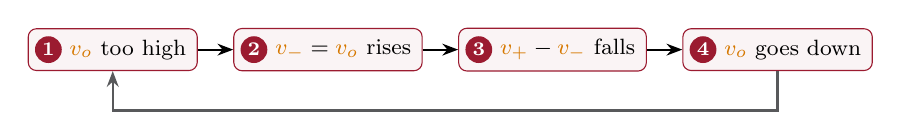
\begin{tikzpicture}[font=\footnotesize, st/.style={draw=metured, rounded corners=3pt, fill=metured!5, inner sep=4pt}]
    \node[st] (a) at (0,0) [label={[cn, label distance=-4.4mm]west:1}] {\hspace{11pt}$\vo$ too high};
    \node[st, anchor=west] (b) at ($(a.east)+(0.45,0)$) [label={[cn, label distance=-4.4mm]west:2}] {\hspace{11pt}$\vm = \vo$ rises};
    \node[st, anchor=west] (c) at ($(b.east)+(0.45,0)$) [label={[cn, label distance=-4.4mm]west:3}] {\hspace{11pt}$\vp - \vm$ falls};
    \node[st, anchor=west] (e) at ($(c.east)+(0.45,0)$) [label={[cn, label distance=-4.4mm]west:4}] {\hspace{11pt}$\vo$ goes down};
    \draw[-{Stealth[length=2mm]}, thick] (a) -- (b);
    \draw[-{Stealth[length=2mm]}, thick] (b) -- (c);
    \draw[-{Stealth[length=2mm]}, thick] (c) -- (e);
    \draw[-{Stealth[length=2mm]}, thick, metugray] (e.south) -- ++(0,-0.5) -| (a.south);
  \end{tikzpicture}}
%  block diagram of the follower: difference operator, op-amp block A, unity feedback
%  #1 = 1: show the numbered steps of the loop
\newcommand{\fbBlock}[1]{%
  \begin{tikzpicture}[font=\small, >={Stealth[length=2.2mm]}]
    \node[draw, circle, thick, minimum size=6.5mm, inner sep=0pt] (s) at (1.2,0) {};
    \node[font=\scriptsize] at ($(s)+(-0.45,0.22)$) {$+$};
    \node[font=\scriptsize] at ($(s)+(0.22,-0.48)$) {$-$};
    \node[draw, thick, fill=metulight, minimum width=1.2cm, minimum height=0.85cm] (b) at (3.4,0) {$A$};
    \node[font=\scriptsize, text=metugray, above] at (b.north) {op-amp};
    \draw[->, thick] (0,0) node[left, text=cvolt] {$v_{\mathrm{in}}$} -- (s.west);
    \draw[->, thick] (s.east) -- (b.west) node[midway, above, text=cvolt] {$v_d$};
    \draw[->, thick] (b.east) -- (5.6,0) node[right, text=cvolt] {$v_o$};
    \fill (4.8,0) circle (1.6pt);
    \draw[->, thick, metured] (4.8,0) -- (4.8,-1.3) -- (1.2,-1.3) -- (s.south);
    \node[font=\small, text=cvolt, anchor=east] at (1.12,-0.85) {$v_-$};
    \ifnum#1=1
      \node[cn] at (5.1,0.33) {1};
      \node[cn] at (1.5,-0.9) {2};
      \node[cn] at (2.4,-0.33) {3};
      \node[cn] at (4.25,0.62) {4};
    \fi
  \end{tikzpicture}}

%  source with internal resistance -> follower -> load, and its equivalent
\newcommand{\bufThev}{%
  \draw (0,1.8) to[american voltage source, l_=$\Vcol{v_s}$] (0,0) node[ground] {};
  \draw (0,1.8) to[R, l=$R_s$] (2.0,1.8) coordinate (p);
  \node[oa, noinv input up, anchor=+] (B) at (2.6,1.8) {};
  \draw (p) -- (B.+);
  \draw (B.out) -- ++(0.7,0) coordinate (fo) -- ++(1.2,0) coordinate (lo);
  \draw (B.-) -- ++(-0.4,0) -- ++(0,-0.8) -| (fo);
  \draw (lo) to[R, l_=$R_L$] (lo |- 0,0) node[ground] {};
  \fill (fo) circle (1.6pt);
  \draw[iar] (0.65,1.45) -- (1.3,1.45); \node[font=\small, text=ccur, below] at (0.97,1.45) {$i_+ = 0$};
  \node[font=\small, text=cvolt] at ($(lo |- 0,0.9)+(0.6,0)$) {$v_s$};
  \node[pol] at ($(lo |- 0,1.4)+(0.6,0)$) {$+$}; \node[pol] at ($(lo |- 0,0.4)+(0.6,0)$) {$-$};}
\newcommand{\bufEquiv}{%
  \draw (0,1.8) to[american voltage source, l_=$\Vcol{v_s}$] (0,0) node[ground] {};
  \draw (0,1.8) -- (1.6,1.8) to[R, l=$R_L$] (1.6,0) -- (0,0);}
\title{Lecture 16: Operational Amplifiers}
\subtitle{EE201 -- Circuit Theory I}
\author{M. Mert Ankaral{\i}}
\institute{\small Department of Electrical and Electronics Engineering\\
           Middle East Technical University}
\date{}

%  Roadmap icons (1-6)
\newcommand{\rmicon}[1]{%
  \ifcase#1\or
    \node[op amp, fill=metulight, thick] (I) at (0,0) {}; \draw (I.out) -- ++(0.4,0);
    \draw (I.up) -- ++(0,0.3); \draw (I.down) -- ++(0,-0.3);
  \or
    \node[op amp, noinv input up, fill=metulight, thick] (I) at (0,0) {};
    \draw (I.+) -- ++(-0.8,0); \draw (I.out) -- ++(0.5,0) coordinate (o);
    \draw[-{Stealth[length=2.2mm]}, thick, metured] (o) -- ++(0,-1.1) -| ($(I.-)+(-0.4,0)$) -- (I.-);
  \or
    \draw[-{Stealth[length=2mm]}] (-1.5,0) -- (1.6,0); \draw[-{Stealth[length=2mm]}] (0,-1.0) -- (0,1.1);
    \draw[metured, very thick] (-1.4,-0.7) -- (0,-0.7) -- (0,0.7) -- (1.4,0.7);
  \or
    \node[op amp, noinv input up, fill=metulight, thick] (I) at (0,0) {};
    \draw (I.+) -- ++(-0.5,0); \draw (I.-) -- ++(-0.2,0) -- ++(0,-0.6) -| (1.4,0) (I.out) -- (1.6,0);
  \or
    \node[op amp, fill=metulight, thick] (I) at (0,0.2) {};
    \draw (I.-) -- ++(-0.3,0) -- ++(0,0.8) to[R] ++(2.4,0) -- ++(0,-0.8) -- (I.out);
  \or
    \node[op amp, fill=metulight, thick] (I) at (0,0.2) {};
    \draw (I.-) -- ++(-0.3,0) -- ++(0,0.8) to[C] ++(2.4,0) -- ++(0,-0.8) -- (I.out);
    \draw (I.-) ++(-0.3,0) to[R] ++(-1.3,0);
  \or
    \draw[-{Stealth[length=2mm]}] (-1.6,0) -- (1.7,0); \draw[-{Stealth[length=2mm]}] (0,-1.0) -- (0,1.1);
    \draw[metured, very thick] (-1.5,-0.7) -- (-0.45,-0.7) -- (0.45,0.7) -- (1.5,0.7);
    \node[font=\Large] at (1.0,0.15) {$A$};
  \fi}
%  Stops 1-14: station of stop k = \rmst{k}
\newcommand{\rmst}[1]{\ifcase#1\or1\or1\or2\or2\or3\or3\or4\or4\or5\or5\or5\or5\or6\or7\fi}
\newcommand{\rmstation}[4]{%
  \ifnum#1<\rmS\relax
    \node[circle, fill=cpow, text=white, inner sep=0pt, minimum size=5.4mm, font=\scriptsize\bfseries] at (#2,0) {\checkmark};
    \node[text=black!40, font=\footnotesize\bfseries, align=center, anchor=south, inner sep=1pt] at (#2,0.36) {#3};
  \else\ifnum#1=\rmS\relax
    \node[circle, fill=metured, text=white, inner sep=0pt, minimum size=6.2mm, font=\small\bfseries] at (#2,0) {#1};
    \node[text=metured, font=\footnotesize\bfseries, align=center, anchor=south, inner sep=1pt] at (#2,0.36) {#3};
  \else
    \node[circle, draw=metugray, fill=white, text=metugray, inner sep=0pt, minimum size=5.4mm, font=\scriptsize\bfseries] at (#2,0) {#1};
    \node[font=\footnotesize\bfseries, align=center, anchor=south, inner sep=1pt] at (#2,0.36) {#3};
  \fi\fi
  \begin{scope}[shift={(#2,1.75)}, scale=0.34, transform shape]
    \ifnum#1>\rmS\relax\begin{scope}[opacity=0.5]\rmicon{#4}\end{scope}\else\rmicon{#4}\fi
  \end{scope}}
%  #1 first stop, #2 last stop covered by this item, #3 x, #4 y, #5 text
\newcommand{\rmsub}[5]{%
  \ifnum#2<\rmcur\relax
    \node[text width=1.66cm, align=center, font=\scriptsize, text=black!40] at (#3,#4) {#5\ \textcolor{cpow}{\checkmark}};
  \else\ifnum#1>\rmcur\relax
    \node[text width=1.66cm, align=center, font=\scriptsize] at (#3,#4) {#5};
  \else
    \node[text width=1.66cm, align=center, font=\scriptsize\bfseries, text=metured,
          draw=metured, rounded corners=2pt, inner sep=2pt] at (#3,#4) {#5};
  \fi\fi}
\newcommand{\roadmapframe}[1]{%
  \begin{frame}{Roadmap}
    \def\rmcur{#1}\edef\rmS{\rmst{#1}}%
    \vfill
    \centering
    \begin{tikzpicture}
      \draw[metugray!45, line width=3pt, -{Stealth[length=2.6mm, width=3.2mm]}] (0,0) -- (13.4,0);
      \rmstation{1}{1.00}{The\\ op-amp}{1}
      \rmstation{2}{2.90}{Feedback}{2}
      \rmstation{3}{4.80}{Ideal\\ model}{3}
      \rmstation{4}{6.70}{Voltage\\ follower}{4}
      \rmstation{5}{8.60}{Amplifiers}{5}
      \rmstation{6}{10.50}{Integrator}{6}
      \rmstation{7}{12.40}{Finite\\ gain}{7}
      \rmsub{1}{1}{1.00}{-0.8}{terminals, regions}
      \rmsub{2}{2}{1.00}{-1.5}{models}
      \rmsub{3}{3}{2.90}{-0.8}{follower, finite $A$}
      \rmsub{4}{4}{2.90}{-1.5}{$v_+ \approx v_-$}
      \rmsub{5}{5}{4.80}{-0.8}{$A \to \infty$}
      \rmsub{6}{6}{4.80}{-1.5}{the method}
      \rmsub{7}{7}{6.70}{-0.8}{buffer}
      \rmsub{8}{8}{6.70}{-1.5}{positive feedback}
      \rmsub{9}{9}{8.60}{-0.8}{inverting}
      \rmsub{10}{10}{8.60}{-1.5}{non-inverting}
      \rmsub{11}{11}{8.60}{-2.1}{summing}
      \rmsub{12}{12}{8.60}{-2.7}{difference}
      \rmsub{13}{13}{10.50}{-0.8}{integrator,\\ differentiator}
      \rmsub{14}{14}{12.40}{-0.8}{inverting amplifier}
    \end{tikzpicture}
    \vfill
    \mbox{}
    \vfill
  \end{frame}}
\newcommand{\qbox}[1]{\begin{tikzpicture}\node[draw=metured, thick, fill=metured!5, rounded corners=3pt, inner sep=5pt] {#1};\end{tikzpicture}}

\begin{document}

%--------------------------------------------------------------
\begin{frame}[plain]
  \titlepage
  \vspace{-1.2em}
  \begin{center}\scriptsize\color{metugray}
    \Icol{$\blacksquare$}~current \quad \Vcol{$\blacksquare$}~voltage \quad
    \textcolor{metured}{$\blacksquare$}~characteristic
  \end{center}
\end{frame}

%--------------------------------------------------------------
\begin{frame}{Review: elements with regions}
  \vfill
  \begin{columns}[c,onlytextwidth]
    \begin{column}{0.44\textwidth}
      \centering
      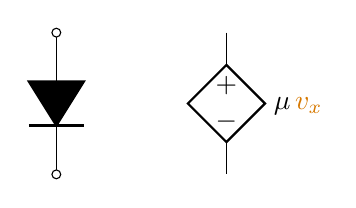
\begin{tikzpicture}[scale=0.9]
        \draw (0,2.0) node[ocirc] {} -- (0,1.7); \draw (0,1.7) to[D*] (0,0.3); \draw (0,0.3) -- (0,0) node[ocirc] {};
        \begin{scope}[xshift=2.4cm]
          \draw (0,2.0) to[american controlled voltage source, l=$\mu\,\Vcol{v_x}$] (0,0);
        \end{scope}
      \end{tikzpicture}
    \end{column}
    \begin{column}{0.54\textwidth}
      \begin{itemize}\itemsep8pt
        \item Ideal diode: two regions, ON and OFF
        \item Method: assume a region, solve, check its condition
        \item Dependent source: a voltage set by another voltage
        \item Today: an element with three regions, built on a dependent source
      \end{itemize}
    \end{column}
  \end{columns}
  \vfill
\end{frame}

%==============================================================
\roadmapframe{1}

%--------------------------------------------------------------
\begin{frame}{Motivation: amplify a difference}
  \vfill
  \begin{columns}[c,onlytextwidth]
    \begin{column}{0.42\textwidth}
      \centering
      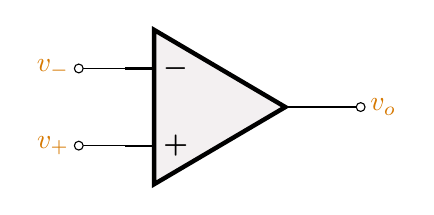
\begin{tikzpicture}[scale=1.0]
        \node[oa] (A) at (0,0) {};
        \draw (A.-) -- ++(-0.6,0) node[ocirc] {} node[left, text=cvolt] {$v_-$};
        \draw (A.+) -- ++(-0.6,0) node[ocirc] {} node[left, text=cvolt] {$v_+$};
        \draw (A.out) -- ++(0.6,0) node[ocirc] {} node[right, text=cvolt] {$v_o$};
      \end{tikzpicture}\\[10pt]
      $\vo \approx 200\,000\,(\Vcol{v_+ - v_-})$
    \end{column}
    \begin{column}{0.56\textwidth}
      \begin{itemize}\itemsep8pt
        \item An integrated circuit: the operational amplifier (op-amp)
        \item A high-gain amplifier of the input difference
        \item Alone: almost any input drives it to its limits
        \item With feedback: exact gains, adders, subtractors, integrators
      \end{itemize}
    \end{column}
  \end{columns}
  \vfill
\end{frame}

%--------------------------------------------------------------
\begin{frame}{Terminals and supplies}
  \vfill
  \begin{columns}[c,onlytextwidth]
    \begin{column}{0.56\textwidth}
      \centering
      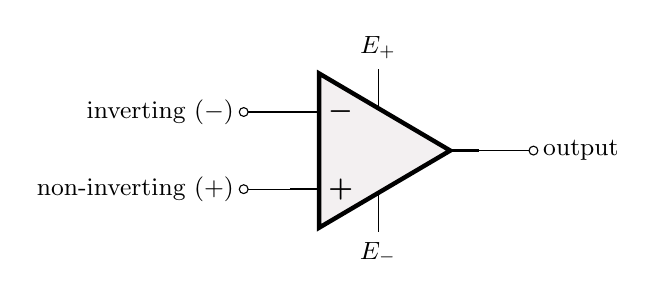
\begin{tikzpicture}[scale=1.0]
        \oaDevice
      \end{tikzpicture}
    \end{column}
    \begin{column}{0.42\textwidth}
      \begin{itemize}\itemsep8pt
        \item Two inputs, one output
        \item Two DC supplies $E_+ > E_-$
        \item Output limits: \ $E_- \leq \vo \leq E_+$
        \item Usually symmetric: \ $\pm\Es$
        \item Voltages w.r.t.\ a common ground
      \end{itemize}
    \end{column}
  \end{columns}
  \vfill
\end{frame}

%--------------------------------------------------------------
\begin{frame}{The transfer characteristic}
  \begin{columns}[c,onlytextwidth]
    \begin{column}{0.5\textwidth}
      \centering
      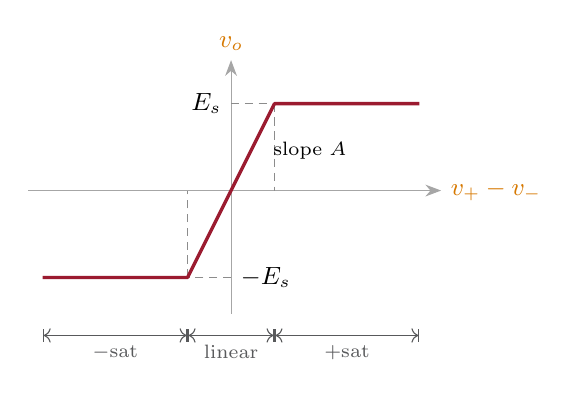
\begin{tikzpicture}[scale=0.92]
        \oaChar{1}
      \end{tikzpicture}
    \end{column}
    \begin{column}{0.48\textwidth}
      \small
      \renewcommand{\arraystretch}{1.3}
      \begin{tabular}{@{}ll@{}}
        \toprule
        linear & $\vo = A\,(\Vcol{v_+ - v_-})$\\
        $+$sat & $\vo = \Es$\\
        $-$sat & $\vo = -\Es$\\
        \bottomrule
      \end{tabular}\\[12pt]
      Open-loop gain $A \approx 2 \times 10^5$\\[6pt]
      \onslide<2->{%
      $\Es = 12\V$: linear only for\\[2pt]
      $|\Vcol{v_+ - v_-}| \leq \dfrac{12}{2 \times 10^5} = 60\,\mu\mathrm{V}$\\[6pt]
      \alert{Open loop: almost always saturated}}
    \end{column}
  \end{columns}
\end{frame}

%--------------------------------------------------------------
\begin{frame}{The dependent-source model}
  \vfill
  \begin{columns}[c,onlytextwidth]
    \begin{column}{0.52\textwidth}
      \centering
      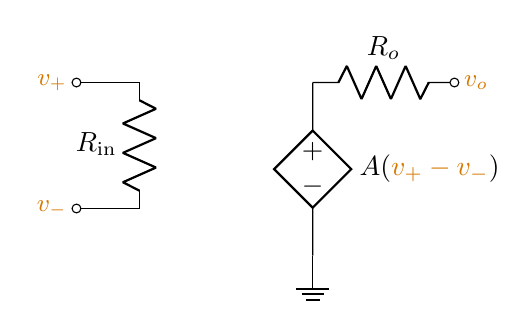
\begin{tikzpicture}[scale=1.0]
        \oaModel
      \end{tikzpicture}
    \end{column}
    \begin{column}{0.46\textwidth}
      \small
      \renewcommand{\arraystretch}{1.35}
      \begin{tabular}{@{}ll@{}}
        \toprule
        input resistance $R_{\mathrm{in}}$ & $10^6$ -- $10^{12}\ohm$\\
        output resistance $R_o$ & $10$ -- $100\ohm$\\
        open-loop gain $A$ & $10^5$ -- $10^8$\\
        \bottomrule
      \end{tabular}\\[14pt]
      Valid in the linear region
    \end{column}
  \end{columns}
  \vfill
\end{frame}

%--------------------------------------------------------------
\begin{frame}{The finite-gain ideal model}
  \vfill
  \begin{columns}[c,onlytextwidth]
    \begin{column}{0.46\textwidth}
      \centering
      \begin{tikzpicture}[scale=1.1]
        \oaFGModel
      \end{tikzpicture}
    \end{column}
    \begin{column}{0.52\textwidth}
      $R_{\mathrm{in}} = \infty$, \ $R_o = 0$\\[8pt]
      $\ip = \im = 0$\\[8pt]
      Linear: \ $\vo = A\,(\vp - \vm)$\\[8pt]
      $A$ is still finite
    \end{column}
  \end{columns}
  \vfill
\end{frame}

%==============================================================
\roadmapframe{3}

%--------------------------------------------------------------
\begin{frame}{Negative feedback: the follower}
  \begin{columns}[c,onlytextwidth]
    \begin{column}{0.44\textwidth}
      \centering
      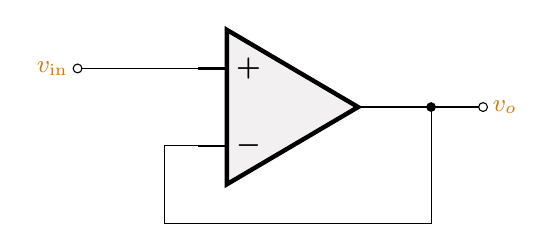
\begin{tikzpicture}[scale=1.1]
        \follower{0}
      \end{tikzpicture}\\[10pt]
      Output back to the $-$ input\\[4pt]
      $\vp = \vin$, \ $\vm = \vo$\\[4pt]
      Finite gain $A$: \ $\vo = \ ?$
    \end{column}
    \begin{column}{0.54\textwidth}
      \onslide<2->{%
      $\vo = A\,(\vin - \vo)$\\[6pt]
      \qbox{$\vo = \dfrac{A}{1 + A}\,\vin$, \quad $\vp - \vm = \dfrac{\vo}{A}$}\\[10pt]
      \small
      $\vin = 1\V$:\\[4pt]
      \renewcommand{\arraystretch}{1.25}
      \begin{tabular}{@{}lll@{}}
        \toprule
        $A$ & $\vo$ & $\vp - \vm$\\
        \midrule
        $10^5$ & $0.99999\V$ & $10\,\mu\mathrm{V}$\\
        $10^6$ & $0.999999\V$ & $1\,\mu\mathrm{V}$\\
        $10^8$ & $0.99999999\V$ & $0.01\,\mu\mathrm{V}$\\
        \bottomrule
      \end{tabular}}
    \end{column}
  \end{columns}
\end{frame}

%--------------------------------------------------------------
\begin{frame}{Why the difference stays small}
  \begin{columns}[c,onlytextwidth]
    \begin{column}{0.34\textwidth}
      \centering
      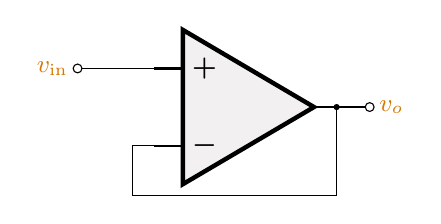
\begin{tikzpicture}[scale=0.7]
        \follower{0}
      \end{tikzpicture}
    \end{column}
    \begin{column}{0.64\textwidth}
      \centering
      \fbBlock{1}
    \end{column}
  \end{columns}
  \vspace{8pt}
  \begin{columns}[t,onlytextwidth]
    \begin{column}{0.5\textwidth}
      \begin{itemize}\itemsep3pt
        \item[\cnum{1}] $\vo$ a little too high
        \item[\cnum{2}] $\vm = \vo$ rises
      \end{itemize}
    \end{column}
    \begin{column}{0.48\textwidth}
      \begin{itemize}\itemsep3pt
        \item[\cnum{3}] $\vp = \vin$ fixed: $\Vcol{v_d}$ falls
        \item[\cnum{4}] $\vo$ goes down
      \end{itemize}
    \end{column}
  \end{columns}
  \vspace{8pt}
  \onslide<2->{%
  \begin{columns}[t,onlytextwidth]
    \begin{column}{0.5\textwidth}
      $\Vcol{v_d} = \vin - \vo$, \ $\vo = A\,\Vcol{v_d}$\\[4pt]
      \qbox{$\Vcol{v_d} = \dfrac{\vin}{1 + A} = \dfrac{\vo}{A} \approx 0$}
    \end{column}
    \begin{column}{0.48\textwidth}
      Open loop: no lower path\\[4pt]
      No correction: saturation\\[4pt]
      \alert{$\vp \approx \vm$ comes from feedback}
    \end{column}
  \end{columns}}
\end{frame}


%==============================================================
\roadmapframe{5}

%--------------------------------------------------------------
\begin{frame}{Let $A \to \infty$}
  \begin{center}
    \fbBlock{0}
  \end{center}
  \vspace{4pt}
  \begin{columns}[t,onlytextwidth]
    \begin{column}{0.5\textwidth}
      Follower, finite $A$:\\[6pt]
      $\vo = \dfrac{A}{1 + A}\,\vin$, \quad $\Vcol{v_d} = \dfrac{\vin}{1 + A}$
    \end{column}
    \begin{column}{0.48\textwidth}
      \onslide<2->{%
      $A \to \infty$:\\[4pt]
      \qbox{$\vo \to \vin$, \quad $\vp - \vm \to 0$}\\[6pt]
      {\small $|\vin| > \Es$: loop cannot zero $\Vcol{v_d}$, saturation}}
    \end{column}
  \end{columns}
\end{frame}

%--------------------------------------------------------------
\begin{frame}{The infinite-gain ideal op-amp}
  \begin{columns}[c,onlytextwidth]
    \begin{column}{0.42\textwidth}
      \centering
      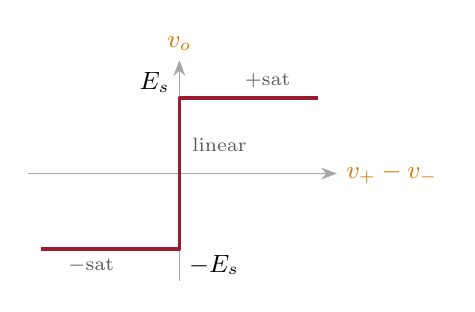
\begin{tikzpicture}[scale=0.8]
        \oaIdealChar
      \end{tikzpicture}\\[8pt]
      \qbox{$\ip = \im = 0$ \ in every region}
    \end{column}
    \begin{column}{0.56\textwidth}
      \centering
      \renewcommand{\arraystretch}{1.35}
      \begin{tabular}{@{}lll@{}}
        \toprule
        linear & $+$sat & $-$sat\\
        \midrule
        $\vp = \vm$ & $\vp > \vm$ & $\vp < \vm$\\
        $|\vo| \leq \Es$ & $\vo = \Es$ & $\vo = -\Es$\\
        \bottomrule
      \end{tabular}\\[12pt]
      \raggedright
      \begin{itemize}\itemsep6pt
        \item $\vp = \vm$: produced by the feedback, not by the op-amp alone
        \item $\vp = \vm$: no connection, no current between the inputs
        \item $\Icol{i_o} \neq 0$: no KCL at the output node
      \end{itemize}
    \end{column}
  \end{columns}
\end{frame}

%--------------------------------------------------------------
\begin{frame}{Analysing an op-amp circuit}
  \vfill
  \begin{enumerate}\itemsep8pt
    \item In every region: KCL at the inputs with $\ip = \im = 0$
    \item \textbf{Linear:} \ $\vp = \vm$, solve for $\vo$, keep $|\vo| \leq \Es$
    \item \textbf{$+$sat:} \ $\vo = \Es$, keep $\vp > \vm$
    \item \textbf{$-$sat:} \ $\vo = -\Es$, keep $\vp < \vm$
    \item Join the pieces: the transfer characteristic
  \end{enumerate}
  \vfill
  \begin{center}
    {\small Like the ideal diode: assume a region, solve, check its condition}
  \end{center}
  \vfill
\end{frame}

%==============================================================
\roadmapframe{7}

%--------------------------------------------------------------
\begin{frame}{The follower with the ideal model}
  \begin{columns}[c,onlytextwidth]
    \begin{column}{0.44\textwidth}
      \centering
      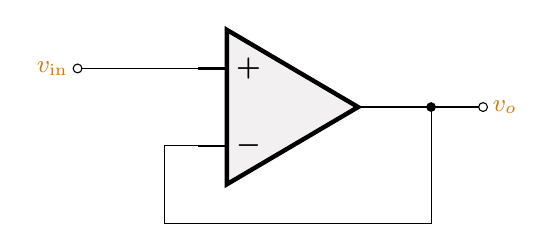
\begin{tikzpicture}[scale=1.1]
        \follower{0}
      \end{tikzpicture}\\[10pt]
      All three regions\\[8pt]
      Every region: \ $\vp = \vin$, \ $\vm = \vo$
    \end{column}
    \begin{column}{0.54\textwidth}
      $\vo = \ ?$\\[6pt]
      \onslide<2->{%
      \small
      Linear: \ $\vo = \vin$, \ $|\vin| \leq \Es$\\[2pt]
      $+$sat: \ $\vp > \vm$: \ $\vin > \Es$\\[2pt]
      $-$sat: \ $\vin < -\Es$\\[4pt]
      \centering
      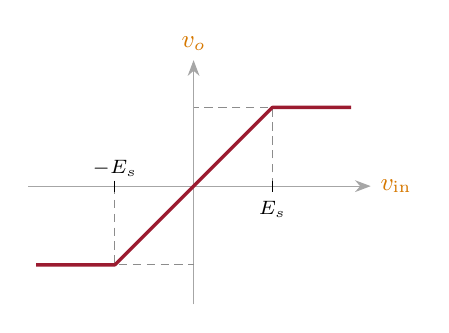
\begin{tikzpicture}[x=0.5cm, y=0.5cm]
        \tax{-4.2}{4.5}{-3.0}{3.2}{$\vin$}{$\vo$}
        \draw[gdash] (2,0) -- (2,2) -- (0,2); \draw[gdash] (-2,0) -- (-2,-2) -- (0,-2);
        \draw[crv] (-4,-2) -- (-2,-2) -- (2,2) -- (4,2);
        \xt{2}{$\Es$} \xtu{-2}{$-\Es$}
      \end{tikzpicture}}
    \end{column}
  \end{columns}
\end{frame}

%--------------------------------------------------------------
\begin{frame}{Why the follower is useful}
  \begin{columns}[c,onlytextwidth]
    \begin{column}{0.62\textwidth}
      \centering
      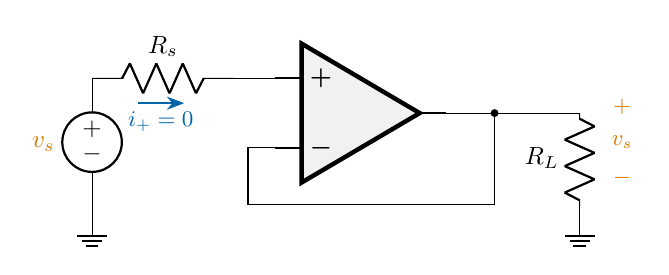
\begin{tikzpicture}[scale=0.9, transform shape]
        \bufThev
      \end{tikzpicture}
    \end{column}
    \begin{column}{0.36\textwidth}
      \centering
      \onslide<2->{%
      $\Longrightarrow$ \quad
      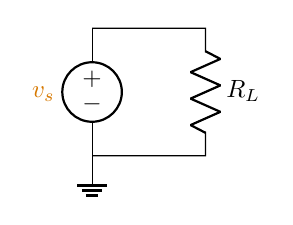
\begin{tikzpicture}[scale=0.9, transform shape, baseline=(current bounding box.center)]
        \bufEquiv
      \end{tikzpicture}}
    \end{column}
  \end{columns}
  \vspace{8pt}
  \begin{itemize}\itemsep4pt
    \item Real source: $\Vcol{v_s}$ with internal $R_s$ (sensor, divider, potentiometer)
    \item Direct load: $\Vcol{v_s}\,R_L/(R_s + R_L)$
    \item<2-> $\ip = 0$: no drop on $R_s$, \ $\vo = \Vcol{v_s}$ for any $R_L$
    \item<2-> Load current from the supplies: source and load isolated
  \end{itemize}
\end{frame}

%--------------------------------------------------------------
\begin{frame}{Example 16.1: loading and buffering}
  \begin{center}
    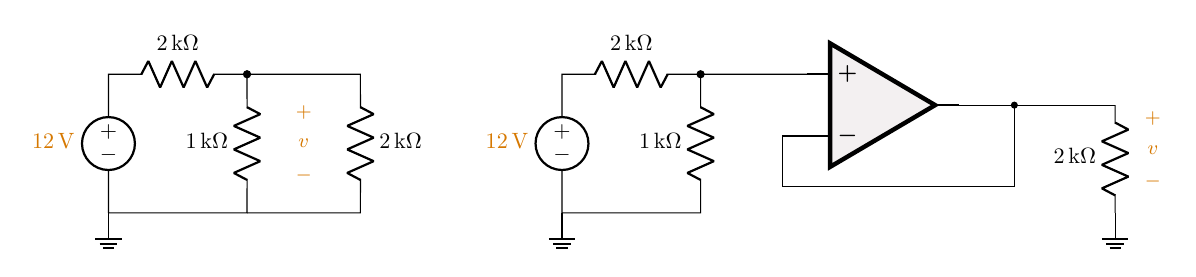
\begin{tikzpicture}[scale=0.8, transform shape]
      \bufEx{0}
      \begin{scope}[xshift=7.2cm] \bufEx{1} \end{scope}
    \end{tikzpicture}
  \end{center}
  \begin{columns}[t,onlytextwidth]
    \begin{column}{0.48\textwidth}
      \centering
      $\Vcol{v} = \ ?$ \ (open circuit: $4\V$)\\[8pt]
      \onslide<2->{%
      $1 \parallel 2 = \tfrac23\kohm$\\[4pt]
      $\Vcol{v} = 12 \cdot \dfrac{2/3}{8/3} = 3\V$: \ \alert{loaded}}
    \end{column}
    \begin{column}{0.48\textwidth}
      \centering
      $\Vcol{v} = \ ?$\\[8pt]
      \onslide<2->{%
      $\ip = 0$: divider unloaded, $\vp = 4\V$\\[4pt]
      $\Vcol{v} = \vo = 4\V$ \ \yes\\[4pt]
      {\small $2\mA$ from the op-amp output}}
    \end{column}
  \end{columns}
\end{frame}

%--------------------------------------------------------------
\begin{frame}{Positive feedback}
  \begin{columns}[c,onlytextwidth]
    \begin{column}{0.4\textwidth}
      \centering
      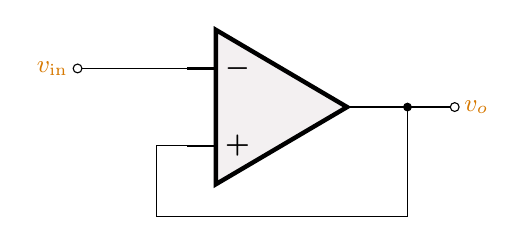
\begin{tikzpicture}[scale=1.0]
        \follower{1}
      \end{tikzpicture}\\[8pt]
      $\vm = \vin$, \ $\vp = \vo$: \ $\vo = \ ?$
    \end{column}
    \begin{column}{0.58\textwidth}
      \onslide<2->{%
      \small
      Linear: $\vo = \vin$, \ $|\vin| \leq \Es$\\
      $+$sat: $\vin < \Es$; \quad $-$sat: $\vin > -\Es$\\[2pt]
      \centering
      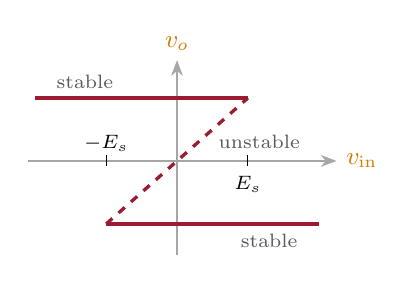
\begin{tikzpicture}[x=0.45cm, y=0.4cm]
        \tax{-4.2}{4.5}{-3.0}{3.2}{$\vin$}{$\vo$}
        \draw[crv] (-4,2) -- (2,2); \draw[crv] (-2,-2) -- (4,-2);
        \draw[crvu] (-2,-2) -- (2,2);
        \xt{2}{$\Es$} \xtu{-2}{$-\Es$}
        \node[reg, above] at (-2.6,2) {stable}; \node[reg, below] at (2.6,-2) {stable};
        \node[reg, anchor=west] at (0.9,0.6) {unstable};
      \end{tikzpicture}}
    \end{column}
  \end{columns}
  \vspace{6pt}
  \onslide<2->{%
  \begin{columns}[t,onlytextwidth]
    \begin{column}{0.48\textwidth}
      \small
      Three solutions; the middle one is unstable\\[2pt]
      $\vo$ up $\to$ $\vp$ up $\to$ $\vo$ further up
    \end{column}
    \begin{column}{0.47\textwidth}
      \small
      \alert{Amplifier: feedback to the $-$ input only}\\[2pt]
      Positive feedback is used on purpose in switching circuits and oscillators (later courses)
    \end{column}
  \end{columns}}
\end{frame}

%==============================================================
\roadmapframe{9}

%--------------------------------------------------------------
\begin{frame}{The inverting amplifier}
  \begin{columns}[c,onlytextwidth]
    \begin{column}{0.46\textwidth}
      \centering
      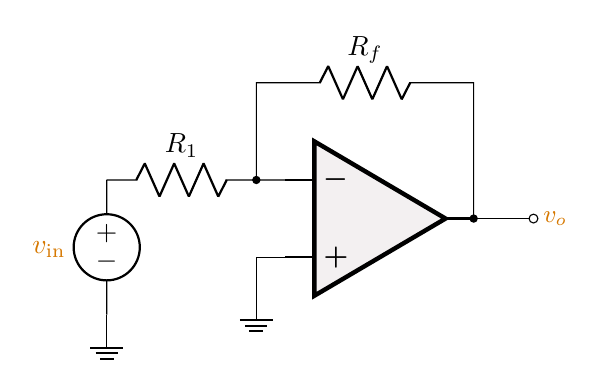
\begin{tikzpicture}[scale=0.95]
        \invAmp{$R_1$}{$R_f$}{$\Vcol{v_{\mathrm{in}}}$}
      \end{tikzpicture}
    \end{column}
    \begin{column}{0.52\textwidth}
      Every region: \ $\vp = 0$\\[4pt]
      KCL ($\im = 0$): \ $\dfrac{\vm - \vin}{R_1} + \dfrac{\vm - \vo}{R_f} = 0$\\[10pt]
      \onslide<2->{%
      Linear: \ $\vm = 0$\\[4pt]
      \qbox{$\vo = -\dfrac{R_f}{R_1}\,\vin$}\\[6pt]
      {\small $|\vin| \leq \dfrac{R_1}{R_f}\Es$; \ $+$sat below, $-$sat above}\\[6pt]
      $\vm = 0$: \textbf{virtual ground}; \ input resistance $R_1$}
    \end{column}
  \end{columns}
\end{frame}

%--------------------------------------------------------------
\begin{frame}{Example 16.2: an inverting amplifier}
  \begin{columns}[c,onlytextwidth]
    \begin{column}{0.46\textwidth}
      \centering
      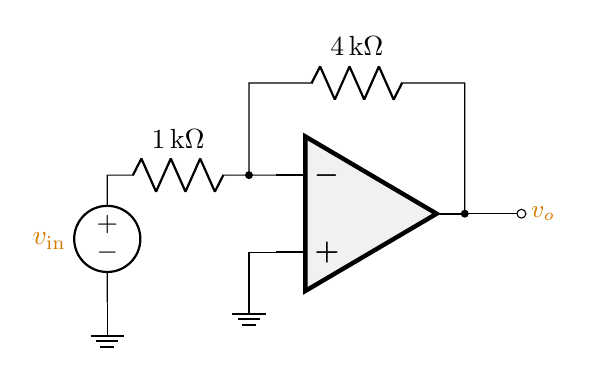
\begin{tikzpicture}[scale=0.9]
        \invAmp{$1\kohm$}{$4\kohm$}{$\Vcol{v_{\mathrm{in}}}$}
      \end{tikzpicture}\\[6pt]
      Supplies $\pm 12\V$\\[4pt]
      $\vo$ for $\vin = 2\V$? \ For $\vin = 5\V$?
    \end{column}
    \begin{column}{0.52\textwidth}
      \centering
      \onslide<2->{%
      Gain $-4$; \ linear for $|\vin| \leq 3\V$\\[4pt]
      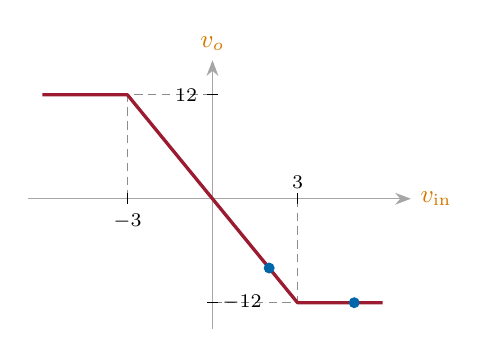
\begin{tikzpicture}[x=0.36cm, y=0.11cm]
        \tax{-6.5}{7}{-15}{16}{$\vin$}{$\vo$}
        \draw[gdash] (3,0) -- (3,-12) -- (0,-12); \draw[gdash] (-3,0) -- (-3,12) -- (0,12);
        \draw[crv] (-6,12) -- (-3,12) -- (3,-12) -- (6,-12);
        \xtu{3}{$3$} \xt{-3}{$-3$} \yt{12}{$12$} \ytr{-12}{$-12$}
        \node[circle, fill=ccur, inner sep=1.4pt] at (2,-8) {}; \node[circle, fill=ccur, inner sep=1.4pt] at (5,-12) {};
      \end{tikzpicture}\\[4pt]
      $\vin = 2\V$: \ $\vo = -8\V$\\[2pt]
      $\vin = 5\V$: \ $-$sat, \ $\vo = -12\V$ \ (not $-20$)}
    \end{column}
  \end{columns}
\end{frame}

%--------------------------------------------------------------
\begin{frame}{The non-inverting amplifier}
  \begin{columns}[c,onlytextwidth]
    \begin{column}{0.46\textwidth}
      \centering
      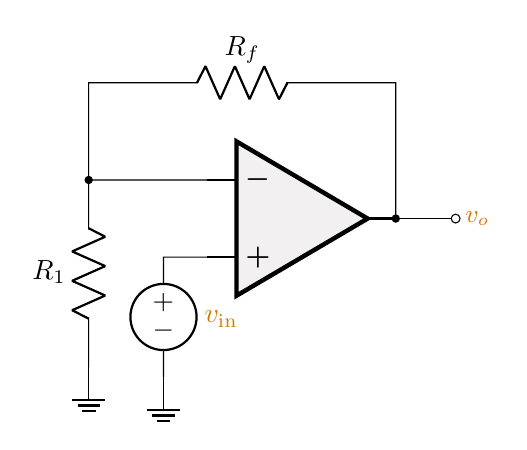
\begin{tikzpicture}[scale=0.95]
        \noninvAmp{$R_1$}{$R_f$}{$\Vcol{v_{\mathrm{in}}}$}
      \end{tikzpicture}
    \end{column}
    \begin{column}{0.52\textwidth}
      Every region: \ $\vp = \vin$\\[4pt]
      Divider ($\im = 0$): \ $\vm = \dfrac{R_1}{R_1 + R_f}\,\vo$\\[10pt]
      \onslide<2->{%
      Linear: \ $\vm = \vp$\\[4pt]
      \qbox{$\vo = \Big(1 + \dfrac{R_f}{R_1}\Big)\vin$}\\[6pt]
      {\small $|\vin| \leq \Es / (1 + R_f/R_1)$}\\[6pt]
      Input draws no current\\[2pt]
      Follower: \ $R_f = 0$, $R_1 = \infty$}
    \end{column}
  \end{columns}
\end{frame}

%--------------------------------------------------------------
\begin{frame}{Example 16.3: a non-inverting amplifier}
  \begin{columns}[c,onlytextwidth]
    \begin{column}{0.46\textwidth}
      \centering
      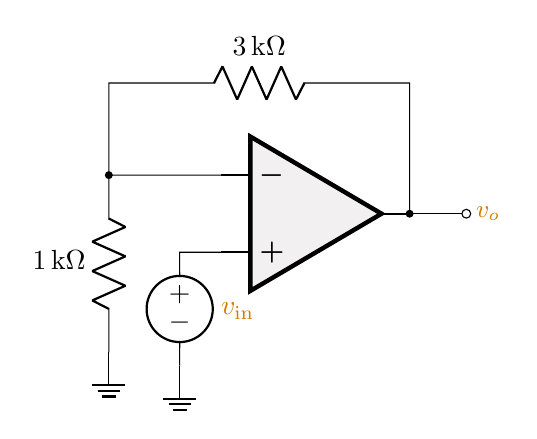
\begin{tikzpicture}[scale=0.9]
        \noninvAmp{$1\kohm$}{$3\kohm$}{$\Vcol{v_{\mathrm{in}}}$}
      \end{tikzpicture}\\[6pt]
      Supplies $\pm 12\V$\\[4pt]
      $\vo$ for $\vin = 1.5\V$? \ For $\vin = -4\V$?
    \end{column}
    \begin{column}{0.52\textwidth}
      \centering
      \onslide<2->{%
      Gain $1 + 3 = 4$; \ linear for $|\vin| \leq 3\V$\\[4pt]
      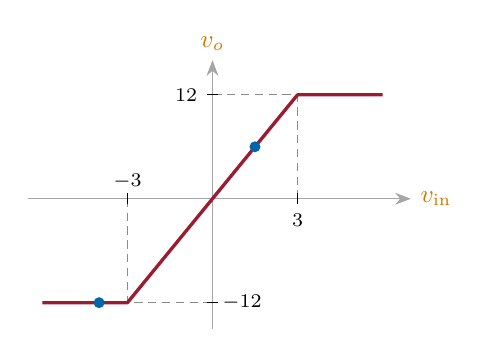
\begin{tikzpicture}[x=0.36cm, y=0.11cm]
        \tax{-6.5}{7}{-15}{16}{$\vin$}{$\vo$}
        \draw[gdash] (3,0) -- (3,12) -- (0,12); \draw[gdash] (-3,0) -- (-3,-12) -- (0,-12);
        \draw[crv] (-6,-12) -- (-3,-12) -- (3,12) -- (6,12);
        \xt{3}{$3$} \xtu{-3}{$-3$} \yt{12}{$12$} \ytr{-12}{$-12$}
        \node[circle, fill=ccur, inner sep=1.4pt] at (1.5,6) {}; \node[circle, fill=ccur, inner sep=1.4pt] at (-4,-12) {};
      \end{tikzpicture}\\[4pt]
      $\vin = 1.5\V$: \ $\vo = 6\V$\\[2pt]
      $\vin = -4\V$: \ $-$sat, \ $\vo = -12\V$}
    \end{column}
  \end{columns}
\end{frame}

%==============================================================
\roadmapframe{11}

%--------------------------------------------------------------
\begin{frame}{The summing amplifier}
  \begin{columns}[c,onlytextwidth]
    \begin{column}{0.48\textwidth}
      \centering
      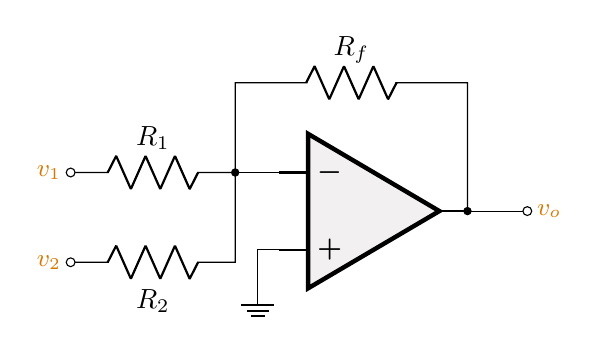
\begin{tikzpicture}[scale=0.95]
        \summing{$R_1$}{$R_2$}{$R_f$}
      \end{tikzpicture}
    \end{column}
    \begin{column}{0.5\textwidth}
      Linear: \ $\vm = \vp = 0$ \ (virtual ground)\\[6pt]
      KCL: \ $\dfrac{\Vcol{v_1}}{R_1} + \dfrac{\Vcol{v_2}}{R_2} = -\dfrac{\vo}{R_f}$\\[10pt]
      \onslide<2->{%
      \qbox{$\vo = -\Big(\dfrac{R_f}{R_1}\Vcol{v_1} + \dfrac{R_f}{R_2}\Vcol{v_2}\Big)$}\\[8pt]
      $n$ inputs: \ $\vo = -\sum_k (R_f/R_k)\,\Vcol{v_k}$\\[4pt]
      {\small Inputs do not affect each other: the node is held at $0\V$}}
    \end{column}
  \end{columns}
\end{frame}

%--------------------------------------------------------------
\begin{frame}{Example 16.4: design an adder}
  \vfill
  \begin{columns}[c,onlytextwidth]
    \begin{column}{0.48\textwidth}
      \centering
      Target: \ $\vo = -(2\,\Vcol{v_1} + \Vcol{v_2})$\\[12pt]
      \onslide<2->{%
      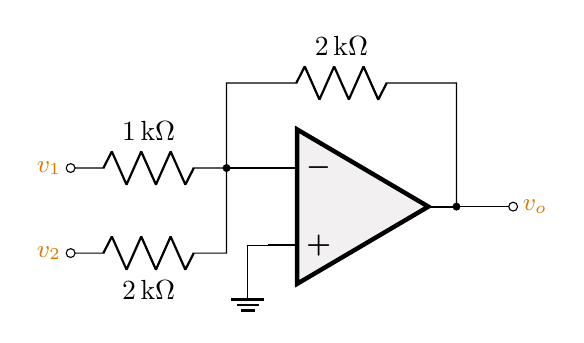
\begin{tikzpicture}[scale=0.9]
        \summing{$1\kohm$}{$2\kohm$}{$2\kohm$}
      \end{tikzpicture}}
    \end{column}
    \begin{column}{0.5\textwidth}
      $R_1, R_2, R_f = \ ?$\\[10pt]
      \onslide<2->{%
      $R_f = 2\kohm$\\[4pt]
      $R_f/R_1 = 2$: \ $R_1 = 1\kohm$\\[4pt]
      $R_f/R_2 = 1$: \ $R_2 = 2\kohm$\\[10pt]
      Check $\Vcol{v_1} = 1\V$, $\Vcol{v_2} = 2\V$:\\[2pt]
      $\vo = -(2 + 2) = -4\V$ \ \yes}
    \end{column}
  \end{columns}
  \vfill
\end{frame}

%--------------------------------------------------------------
\begin{frame}{The difference amplifier}
  \begin{columns}[c,onlytextwidth]
    \begin{column}{0.42\textwidth}
      \centering
      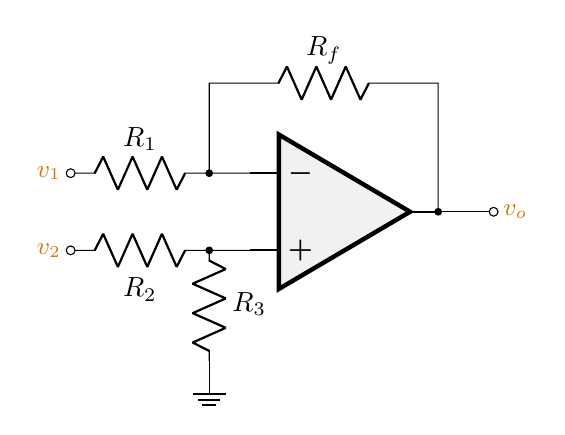
\begin{tikzpicture}[scale=0.88]
        \difference{$R_1$}{$R_2$}{$R_3$}{$R_f$}
      \end{tikzpicture}
    \end{column}
    \begin{column}{0.56\textwidth}
      \small
      Divider: \ $\vp = \dfrac{R_3}{R_2 + R_3}\,\Vcol{v_2}$\\[4pt]
      KCL: \ $\vm = \dfrac{R_f\,\Vcol{v_1} + R_1\,\vo}{R_1 + R_f}$\\[8pt]
      \onslide<2->{%
      Linear, $\vm = \vp$:\\[2pt]
      $\vo = \Big(1 + \dfrac{R_f}{R_1}\Big)\dfrac{R_3}{R_2 + R_3}\Vcol{v_2} - \dfrac{R_f}{R_1}\Vcol{v_1}$\\[8pt]
      \normalsize
      Choose $\dfrac{R_f}{R_1} = \dfrac{R_3}{R_2}$: \ \qbox{$\vo = \dfrac{R_f}{R_1}(\Vcol{v_2} - \Vcol{v_1})$}}
    \end{column}
  \end{columns}
\end{frame}

%--------------------------------------------------------------
\begin{frame}{Example 16.5: a difference amplifier}
  \vfill
  \begin{columns}[c,onlytextwidth]
    \begin{column}{0.48\textwidth}
      \centering
      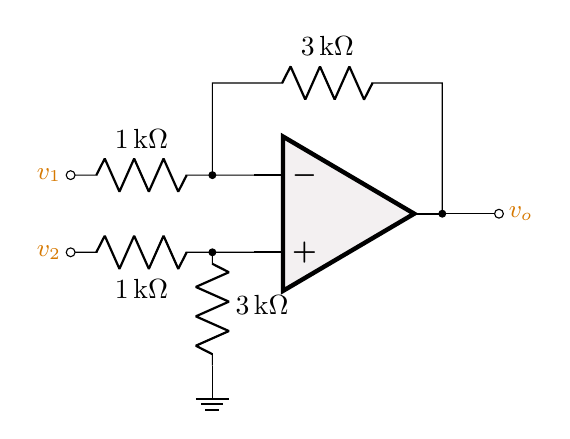
\begin{tikzpicture}[scale=0.9]
        \difference{$1\kohm$}{$1\kohm$}{$3\kohm$}{$3\kohm$}
      \end{tikzpicture}
    \end{column}
    \begin{column}{0.5\textwidth}
      $\vo$ for $\Vcol{v_1} = 2\V$, $\Vcol{v_2} = 3\V$?\\[2pt]
      $\vo$ for $\Vcol{v_1} = \Vcol{v_2} = 5\V$?\\[12pt]
      \onslide<2->{%
      $R_f/R_1 = 3 = R_3/R_2$: \ $\vo = 3\,(\Vcol{v_2} - \Vcol{v_1})$\\[6pt]
      $\vo = 3\,(3 - 2) = 3\V$\\[4pt]
      Equal inputs: \ $\vo = 0$\\[2pt]
      {\small A common voltage is rejected}}
    \end{column}
  \end{columns}
  \vfill
\end{frame}

%==============================================================
\roadmapframe{13}

%--------------------------------------------------------------
\begin{frame}{The integrator}
  \begin{columns}[c,onlytextwidth]
    \begin{column}{0.46\textwidth}
      \centering
      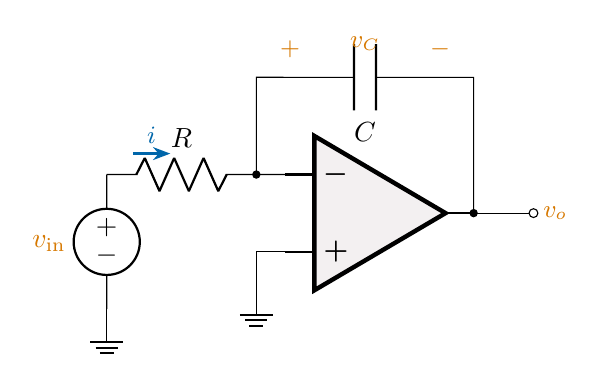
\begin{tikzpicture}[scale=0.95]
        \intdiff{0}
      \end{tikzpicture}\\[6pt]
      {\small Capacitor: \ $\Icol{i} = C\,d\Vcol{v_C}/dt$}
    \end{column}
    \begin{column}{0.52\textwidth}
      Linear: \ $\vm = 0$\\[4pt]
      $\Icol{i} = \dfrac{\vin}{R}$, \qquad $\Vcol{v_C} = -\vo$\\[10pt]
      \onslide<2->{%
      $\Vcol{v_C}(t) = \Vcol{v_C}(0) + \dfrac{1}{C}\displaystyle\int_0^t \Icol{i}\,d\tau$\\[10pt]
      \qbox{$\vo(t) = \vo(0) - \dfrac{1}{RC}\displaystyle\int_0^t \vin(\tau)\,d\tau$}}
    \end{column}
  \end{columns}
\end{frame}

%--------------------------------------------------------------
\begin{frame}{Example 16.6: an integrator saturates}
  \begin{columns}[c,onlytextwidth]
    \begin{column}{0.46\textwidth}
      \centering
      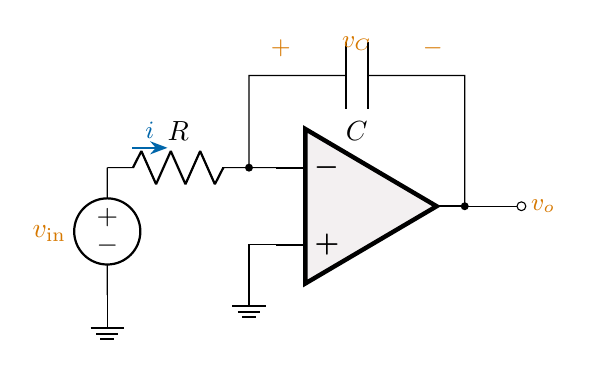
\begin{tikzpicture}[scale=0.9]
        \intdiff{0}
      \end{tikzpicture}\\[6pt]
      $R = 1\kohm$, \ $C = 1\mF$: \ $RC = 1\s$\\[2pt]
      Supplies $\pm 12\V$, \ $\vo(0) = 0$\\[2pt]
      $\vin = 2\V$ from $t = 0$: \ $\vo(t) = \ ?$
    \end{column}
    \begin{column}{0.52\textwidth}
      \centering
      \onslide<2->{%
      $\vo(t) = -\displaystyle\int_0^t 2\,d\tau = -2t$ V\\[8pt]
      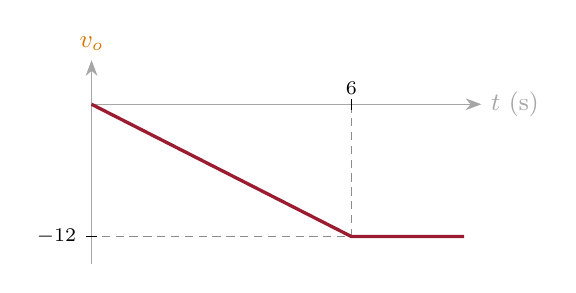
\begin{tikzpicture}[x=0.55cm, y=0.14cm]
        \draw[vax] (0,0) -- (9,0) node[right, font=\small] {$t$ (s)};
        \draw[vax] (0,-14.5) -- (0,4) node[above, font=\small] {$\vo$};
        \draw[gdash] (6,0) -- (6,-12) -- (0,-12);
        \draw[crv] (0,0) -- (6,-12) -- (8.6,-12);
        \xtu{6}{$6$} \yt{-12}{$-12$}
      \end{tikzpicture}\\[6pt]
      $-12\V$ at $t = 6\s$: \ then $-$sat}
    \end{column}
  \end{columns}
\end{frame}

%--------------------------------------------------------------
\begin{frame}{The differentiator}
  \begin{columns}[c,onlytextwidth]
    \begin{column}{0.46\textwidth}
      \centering
      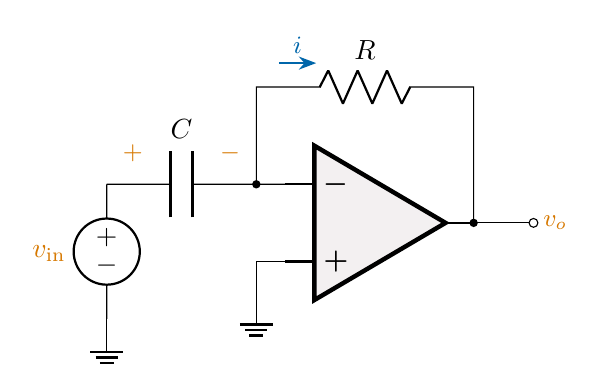
\begin{tikzpicture}[scale=0.95]
        \intdiff{1}
      \end{tikzpicture}
    \end{column}
    \begin{column}{0.52\textwidth}
      Linear: \ $\vm = 0$, \ $\Vcol{v_C} = \vin$\\[4pt]
      $\Icol{i} = C\,\dfrac{d\vin}{dt}$, \qquad $\vo = -R\,\Icol{i}$\\[10pt]
      \onslide<2->{%
      \qbox{$\vo(t) = -RC\,\dfrac{d\vin}{dt}$}\\[10pt]
      $RC = 1\s$, \ $\vin = 3t$ V: \ $\vo = -3\V$}
    \end{column}
  \end{columns}
\end{frame}

%==============================================================
\roadmapframe{14}

%--------------------------------------------------------------
\begin{frame}{Example 16.7: inverting amplifier with finite gain}
  \vfill
  \begin{columns}[c,onlytextwidth]
    \begin{column}{0.46\textwidth}
      \centering
      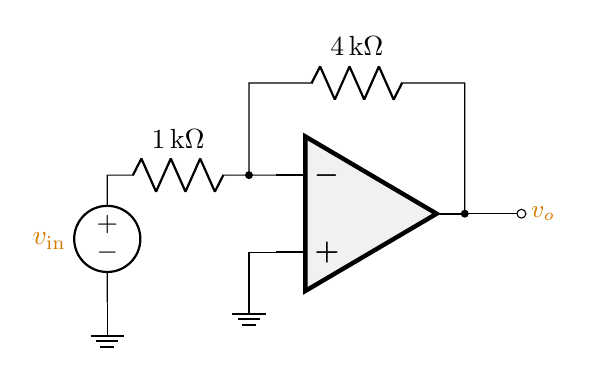
\begin{tikzpicture}[scale=0.9]
        \invAmp{$1\kohm$}{$4\kohm$}{$\Vcol{v_{\mathrm{in}}}$}
      \end{tikzpicture}\\[6pt]
      Finite gain $A = 10^5$: \ $\vo/\vin = \ ?$\\[2pt]
      {\small Ideal: $-4$}
    \end{column}
    \begin{column}{0.52\textwidth}
      \onslide<2->{%
      $\vo = -A\,\vm$\\[4pt]
      KCL: \ $\vm = \dfrac{4\,\vin + \vo}{5}$\\[8pt]
      $\dfrac{\vo}{\vin} = -\dfrac{4}{1 + 5/A} = -3.9998$\\[8pt]
      Error $5/A = 0.005\%$\\[2pt]
      {\small Resistor tolerances matter more}}
    \end{column}
  \end{columns}
  \vfill
\end{frame}

%--------------------------------------------------------------
\begin{frame}{Summary}
  \footnotesize
  \renewcommand{\arraystretch}{1.2}
  \begin{tabular}{@{}>{\raggedright}p{3.2cm} >{\raggedright\arraybackslash}p{9.8cm}@{}}
    \toprule
    negative feedback & follower $A/(1+A)$; \ $\vp - \vm = \vo/A \approx 0$\\
    ideal op-amp & $\ip = \im = 0$; \ linear $\vp = \vm$; \ $\pm$sat $\vo = \pm\Es$\\
    method & every region, then linear, $+$sat, $-$sat with their conditions\\
    follower & $\vo = \vin$: a buffer\\
    inverting, non-inverting & $\vo = -(R_f/R_1)\,\vin$; \ $\vo = (1 + R_f/R_1)\,\vin$\\
    summing, difference & $\vo = -\sum_k (R_f/R_k)\,\Vcol{v_k}$; \ $\vo = (R_f/R_1)(\Vcol{v_2} - \Vcol{v_1})$\\
    integrator, differentiator & $\vo = \vo(0) - \frac{1}{RC}\int_0^t \vin\,d\tau$; \ $\vo = -RC\,d\vin/dt$\\
    positive feedback & linear solution unstable: avoid in amplifiers\\
    finite gain & inverting gain error $\approx (1 + R_f/R_1)/A$\\
    \bottomrule
  \end{tabular}
\end{frame}

\end{document}
